\documentclass[french]{article}
\usepackage[T1]{fontenc}
\usepackage[utf8]{inputenc}
\usepackage{lmodern}
\usepackage[a4paper]{geometry}
\usepackage{graphicx}
\usepackage{hyperref}
\usepackage{hyperref}
\hypersetup{
	colorlinks,
	citecolor=black,
	filecolor=black,
	linkcolor=black,
	urlcolor=black
}
\usepackage{babel}


\newcommand{\fx}{\emph{JavaFX}}
\newcommand{\java}{\emph{Java} }
\newcommand{\himalaya}{\emph{Himalaya} }

% Title Page

\title{{\Huge Himalaya} \\ Rapport de projet}
\author{Sébastien Schouteeten \& Alexis Jouin}

\begin{document}
\begin{figure}
	\centering
	
\includegraphics[width=0.5\linewidth]{images/ulco}
\end{figure}

\maketitle

\begin{figure}
	\centering
	
\includegraphics[width=0.5\linewidth]{images/himalaya}
\end{figure}

\newpage

\tableofcontents

\newpage

\section{Remerciements}
Nous tenons à remercier notre enseignant tuteur, Monsieur Cyril Fonlupt, pour son aide pour le bon déroulement de notre projet. Remerciements également à monsieur Sébastien Verel et monsieur Fabien Teytaud pour les cours de recherches opérationnels et apprentissage artificiel, qui nous a apporté une aide précieuse pour le bon déroulement du projet.

\newpage

\section{Introduction}
Le projet de fin d'année de Master \emph{ISIDIS} est très intéressant et important pour nous initier à un travail de recherche.
Nous avons fait le choix de travailler sur le projet \himalaya en binôme, ce qui implique tout de même une organisation dans les tâches de travaux.
On a fait ce choix, car nous étions intéressés de développer un bot en \java pour un jeu de société.
De plus, ce projet nous a permis d’utiliser de nouvelles technologies que nous ne maîtrisions pas comme \fx.
Notre binôme est composé Sébastien Schouteeten et Alexis Jouin.
À partir de ce constat, nous avons donc essayé de réaliser un logiciel fonctionnel, remplissant les conditions imposées par le cahier des charges validé par monsieur Fonlupt. Nous allons donc voir à travers ce rapport dans une première partie, une présentation du projet ainsi que ses principaux objectifs. Puis dans une seconde partie, les méthodes que nous avons utilisées afin de mettre en \oe uvre le projet et son élaboration. Enfin, dans la dernière partie, nous verrons les résultats obtenus ainsi que les évolutions possibles du projet et plus particulièrement du logiciel.

\newpage

\section{Étude du projet}
\subsection{Contraintes et situations initiales}
Le projet initial à réaliser est un bot en \java pour le jeu de société \himalaya. Le moteur du jeu a déjà été réalisé par l'Université de Nice. Cependant, pour des raisons techniques et pratiques nous avons dû repartir à zéro afin de construire un moteur de jeu plus adapté pour une interface graphique (avec \fx) et les intelligences artificielles. Nous nous sommes tout de même inspirés du travail réalisé précédemment.

\subsection{Pourquoi \fx ?}
\fx contient des outils et composants graphiques les plus maintenus du langage \java.
De plus, cette <<API>> est très rapide et simple à utiliser.
Cela nous a permis en plus d’apprendre et de maitriser un nouvel outil de développement d’interface graphique en \java.

\subsection{Objectifs à réaliser}
Les objectifs principaux du projet ont été de :
\begin{itemize} 
	\item Construire le moteur du jeu 
	\item Construire l'interface graphique
	\item Construire l’intelligence artificielle du jeu
\end{itemize}


\newpage

\section{Élaboration du projet}

\subsection{Les différentes phases du projet}
	\subsubsection{Création du moteur du jeu}
		
		Nous avons débuté le projet par la création du moteur du jeu.
		Ce moteur a été pensé à l'avance avec la réalisation de l'\emph{UML},
		représentant les classes \java.
		Nous nous sommes également aidés du code source du jeu qui nous a été fourni
		en début de projet.
		
		Le moteur du jeu est réalisé de manière à pouvoir être utilisé aussi bien en
		console (terminal), qu'avec une interface graphique.
		
		Durant la réalisation du moteur, nous avons mis en place des tests unitaires,
		dans le but de pouvoir tester notre code, et vérifier qu'aucune des
		fonctionnalités précédentes n'est altérée par les nouvelles.
		
		Nous avons réalisé une classe \emph{Player.java} qui représente un joueur humain,
		et nous avons créé ses classes filles pour utiliser les intelligences artificielles.
		
	\subsubsection{Création de l'interface}
	
		Une fois le moteur terminé et les tests unitaires finis, nous avons réalisé une interface en console.
		Cette dernière nous a permis de réaliser des tests avec une vraie personne qui joue, et de 
		commencer à mettre en place une intelligence artificielle.
		
		Par la suite, nous avons commencé à travailler sur une interface graphique
		du jeu. Nous avons choisi d'utiliser \fx pour réaliser cette étape, car c'est
		la méthode la plus rapide pour mettre en place une interface fonctionnelle en \java.
		En effet, \fx est maintenant la bibliothèque de création d'interfaces graphiques officielle du langage \java.
		
		Nous avons réalisé un menu \reference{menu}, qui permet de sélectionner les joueurs et leur type (Humain, IA aléatoire ou Évolutionnaire). Il est possible, depuis ce menu, de passer en mode 3 ou 4 joueurs.
		
		Juste avant de pouvoir jouer, le jeu demande aux joueurs de choisir leur position de départ \reference{pos_init}.
		
		Durant le déroulement du jeu, nous affichons le plateau ainsi que les ressources
		possédées pour chaque joueur, ainsi que les commandes et ressources proposées sur
		les villages. Les pions des joueurs ainsi que les délégations et stupas qu'ils ont posés
		apparaissent également sur le plateau de jeu \reference{etat_jeu}.
		
		La sélection des actions est effectuée dans une nouvelle fenêtre \reference{actions}, dans laquelle
		le joueur va pouvoir sélectionner les 6 actions qu'il veut effectuer, ainsi que
		la choix de la région s'il choisit de poser une délégation.
		
		À la fin de la partie, une fenêtre s'ouvre et affiche les scores de chaque joueur
		dans chacun des domaines (Politique, Religieux et Économique), ainsi que le vainqueur \reference{resultats}.
			
	\subsubsection{Création des intelligences artificielles}
	
		Nous avons tout d'abord réalisé une IA aléatoire, dans un but de rapidité et de test.
		En effet, celle-ci nous a permis de réaliser une partie, et de vérifier que les différentes actions 
		s'effectuent correctement. Elle choisit 6 actions de manière aléatoire.
		Cette IA a été utile pour tester l'affichage de l'interface graphique, et sa
		mise à jour durant l'exécution des tours : les actions sont effectuées une
		à une, avec une courte pause entre chaque, pour permettre de bien suivre le déroulement du jeu.
		
		Nous avons ensuite commencé le développement de l'IA basée sur un algorithme évolutionnaire.
		Cette dernière utilise l'algorithme évolutionnaire pour réaliser deux choses différentes:
		\begin{itemize}
			\item Choisir sa position de départ.
			\item Planifier les actions qu'elle va réaliser durant le tour.
		\end{itemize}
		
		L'algorithme va réaliser, pour chaque génération, une suite d'actions:
		\begin{enumerate}
			\item Une sélection: on sélectionne les individus qui vont participer à la reproduction.
			\item Des mutations de la population des enfants: mutation ou crossing-over, suivant un ratio donné.
			\item Évaluer la population des enfants, en calculant leur fitness.
			\item effectuer un remplacement: on garde les meilleurs individus pour composer la nouvelle population de parents.
		\end{enumerate}
		
		\lstinputlisting[language=Java, frame=tb, caption= {Déroulement de l'algorithme évolutionnaire}]{code/algo_evol.java}

\newpage

\section{Résultats et perspectives}
\subsection{Résultat final}
\subsection{Améliorations possibles}

\newpage

\section{Conclusion}

\newpage

\section{Annexes}

\begin{figure}[h]
	\centering
	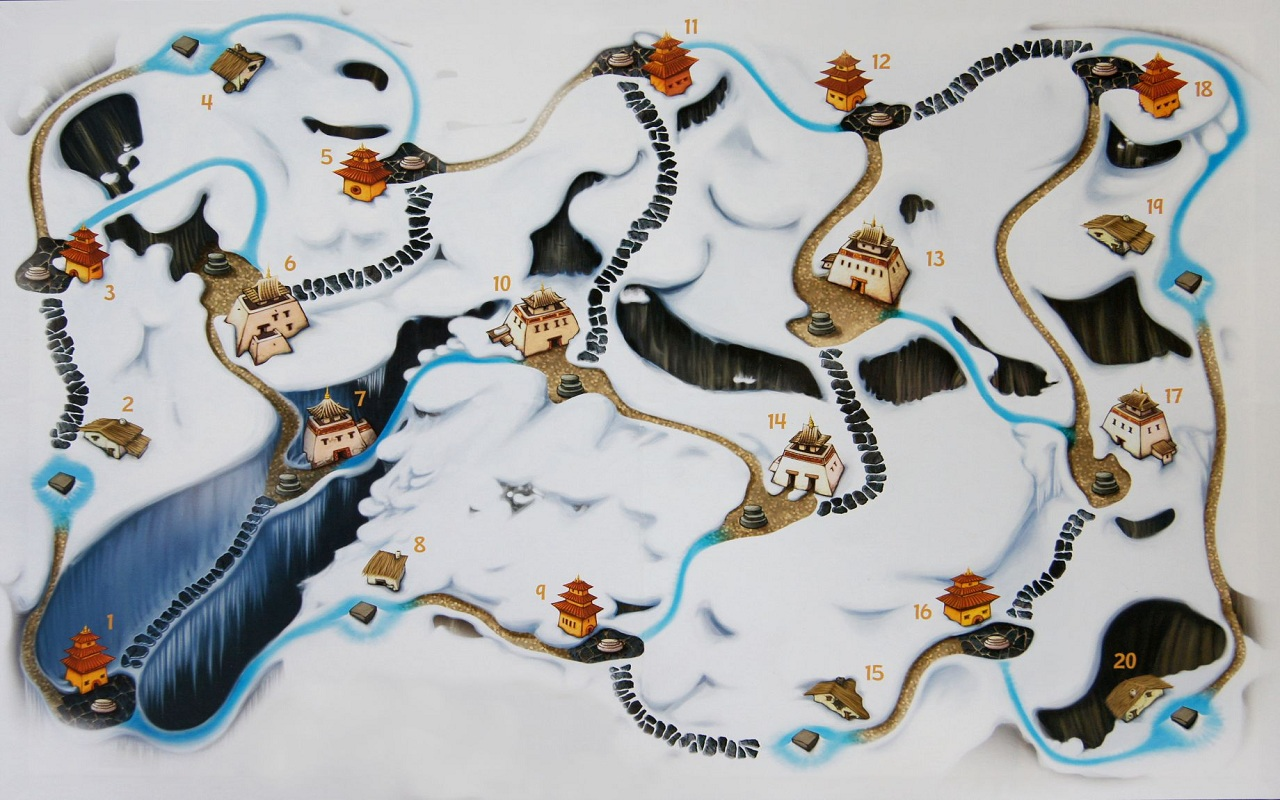
\includegraphics[width=0.7\linewidth]{images/plateau}
	\caption{Plateau du jeu}
	\label{fig:plateau}
\end{figure}

\begin{figure}[h]
	\centering
	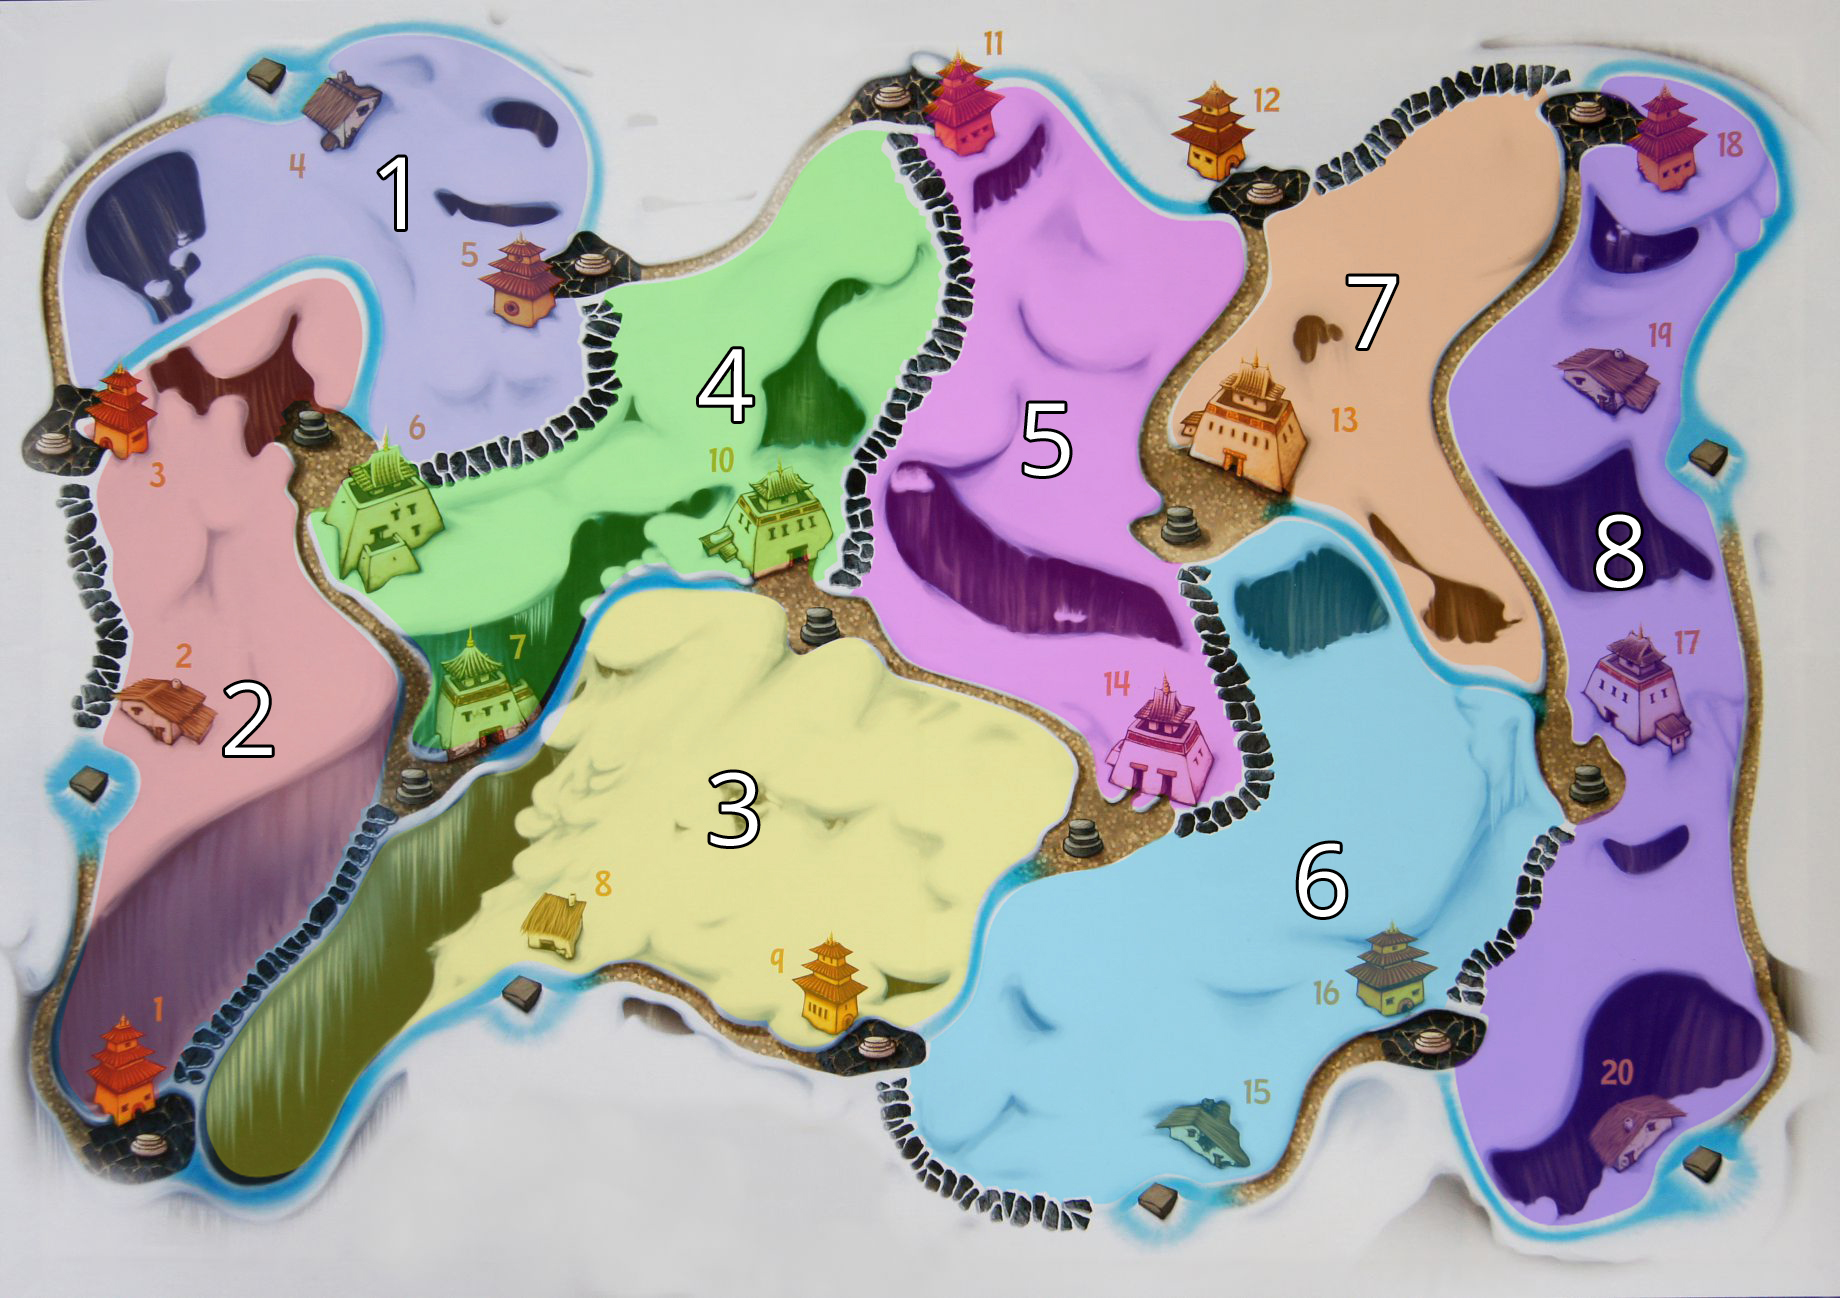
\includegraphics[width=0.7\linewidth]{images/board_regions}
	\caption{Répartitions des régions}
	\label{fig:board_region}
\end{figure}

\begin{figure}[h]
	\centering
	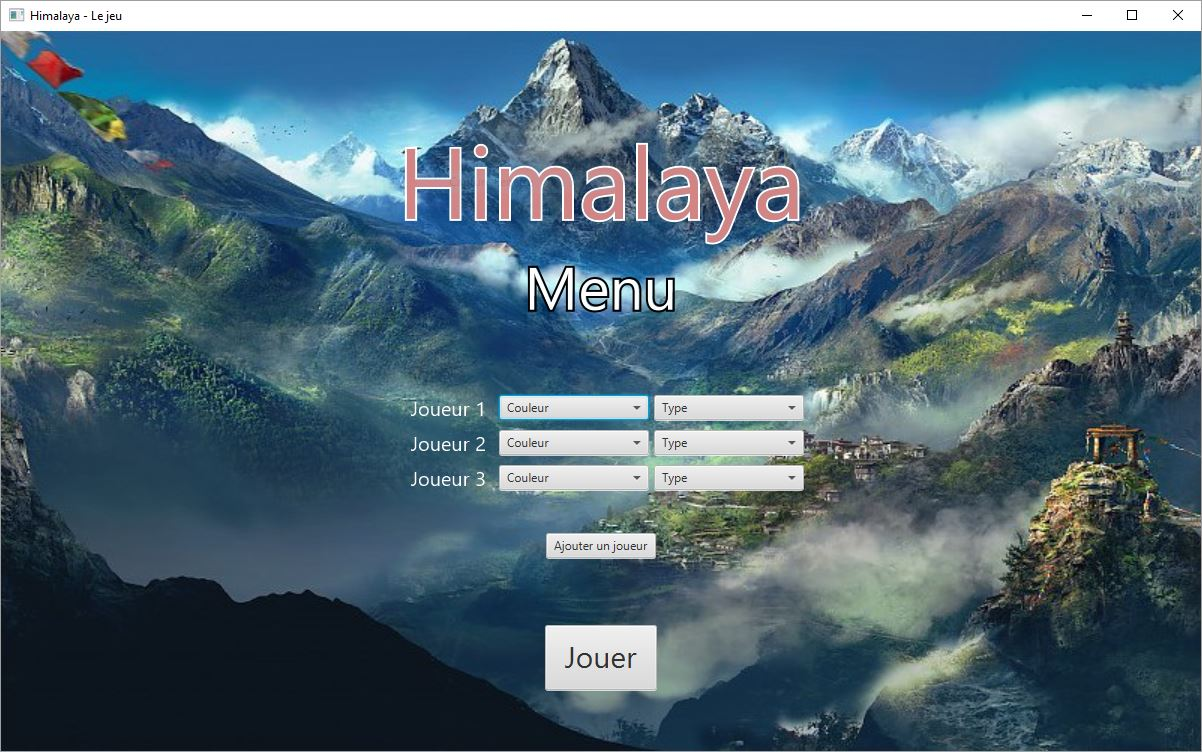
\includegraphics[width=0.9\linewidth]{images/menu}
	\caption{Menu du jeu}
	\label{fig:menu}
\end{figure}

\begin{figure}[h]
	\centering
	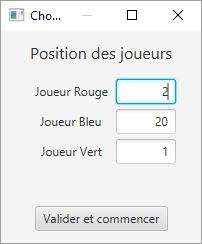
\includegraphics[width=0.4\linewidth]{images/position}
	\caption{Positions initiales}
	\label{fig:pos_init}
\end{figure}

\begin{figure}[h]
	\centering
	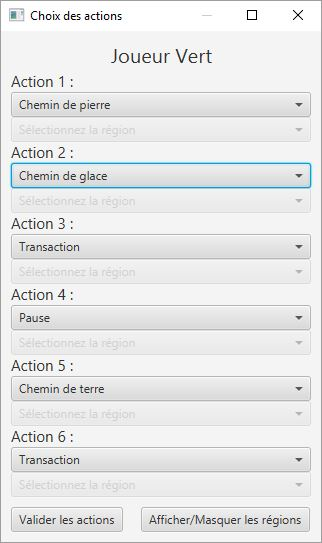
\includegraphics[width=0.4\linewidth]{images/actions}
	\caption{Choix des actions (joueur humain)}
	\label{fig:actions}
\end{figure}

\begin{figure}[h]
	\centering
	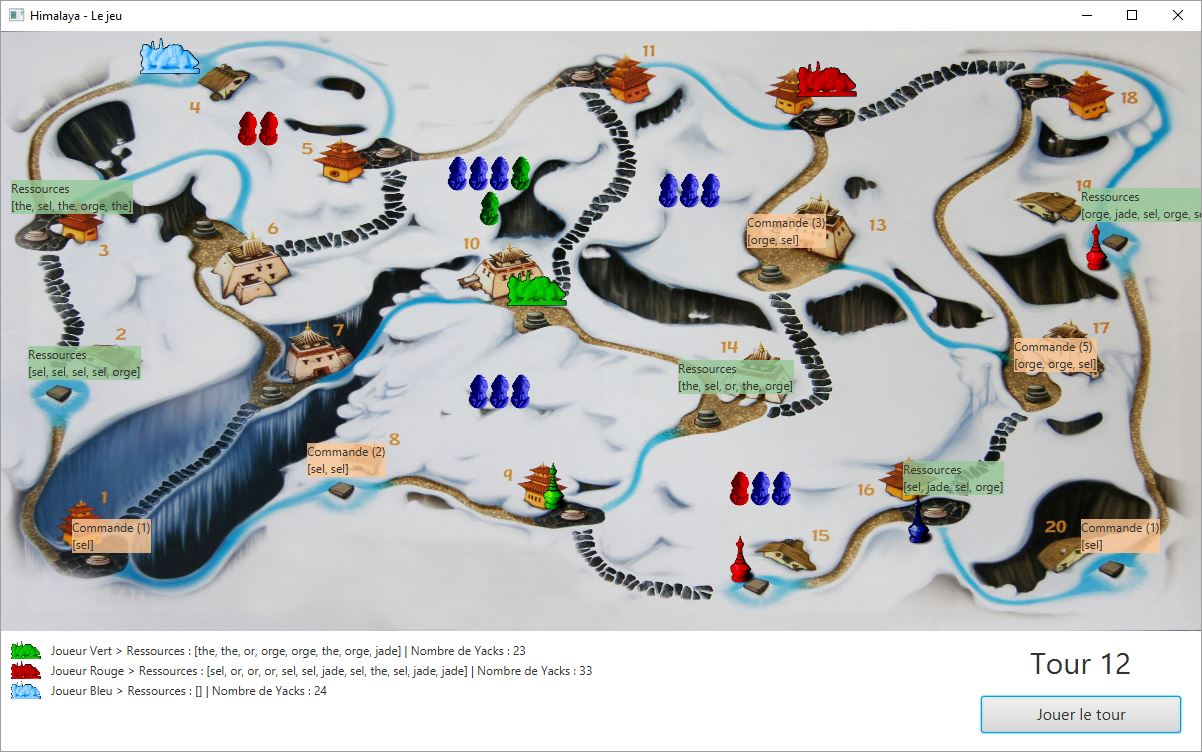
\includegraphics[width=0.9\linewidth]{images/etat_jeu_avance}
	\caption{Déroulement du jeu}
	\label{fig:etat_jeu}
\end{figure}

\begin{figure}[h]
	\centering
	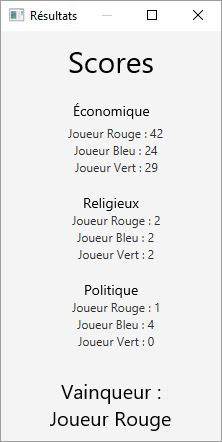
\includegraphics[width=0.3\linewidth]{images/resultats}
	\caption{Résultats de la partie}
	\label{fig:resultats}
\end{figure}

\begin{figure}[h]
	\centering
	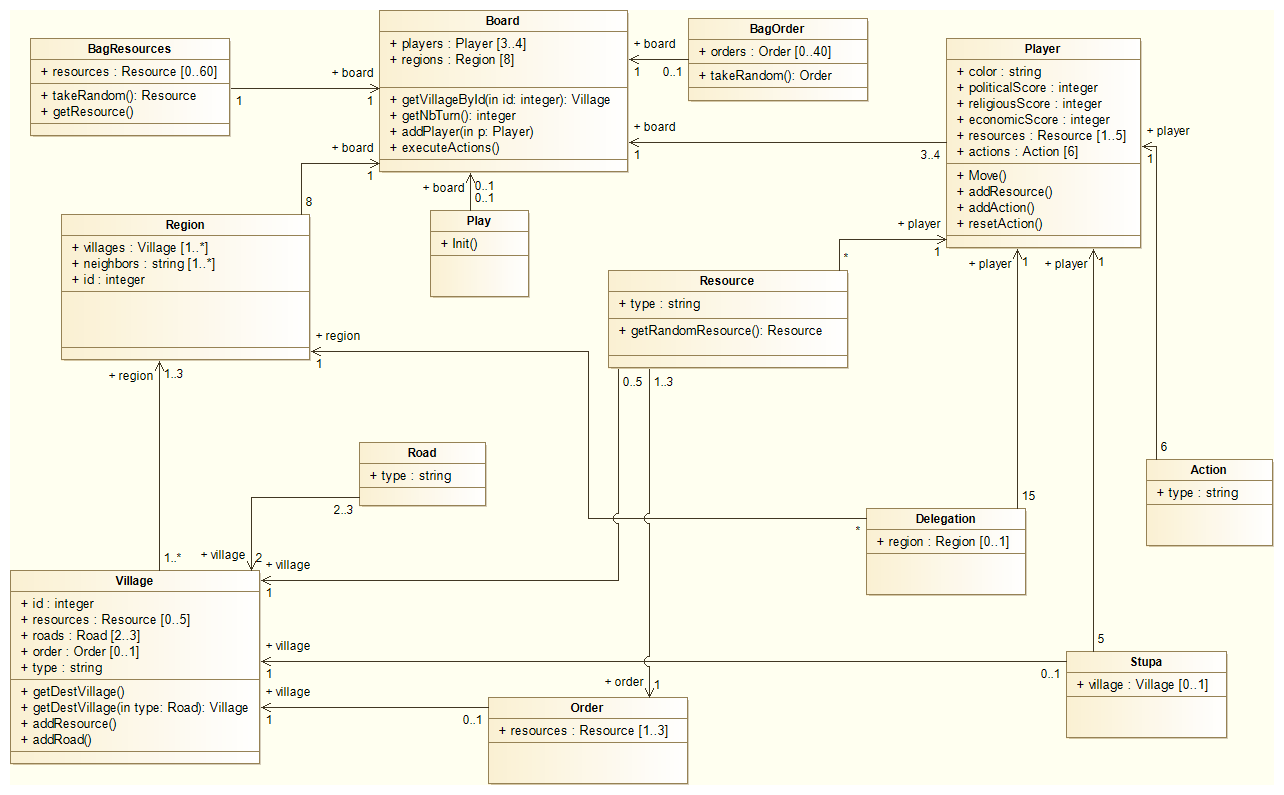
\includegraphics[width=1\linewidth]{images/UML_Himalaya_2}
	\caption{UML Moteur du jeu version 2.5 avant développement}
	\label{fig:UMLCore1}
\end{figure}
\begin{figure}[h]
	\centering
	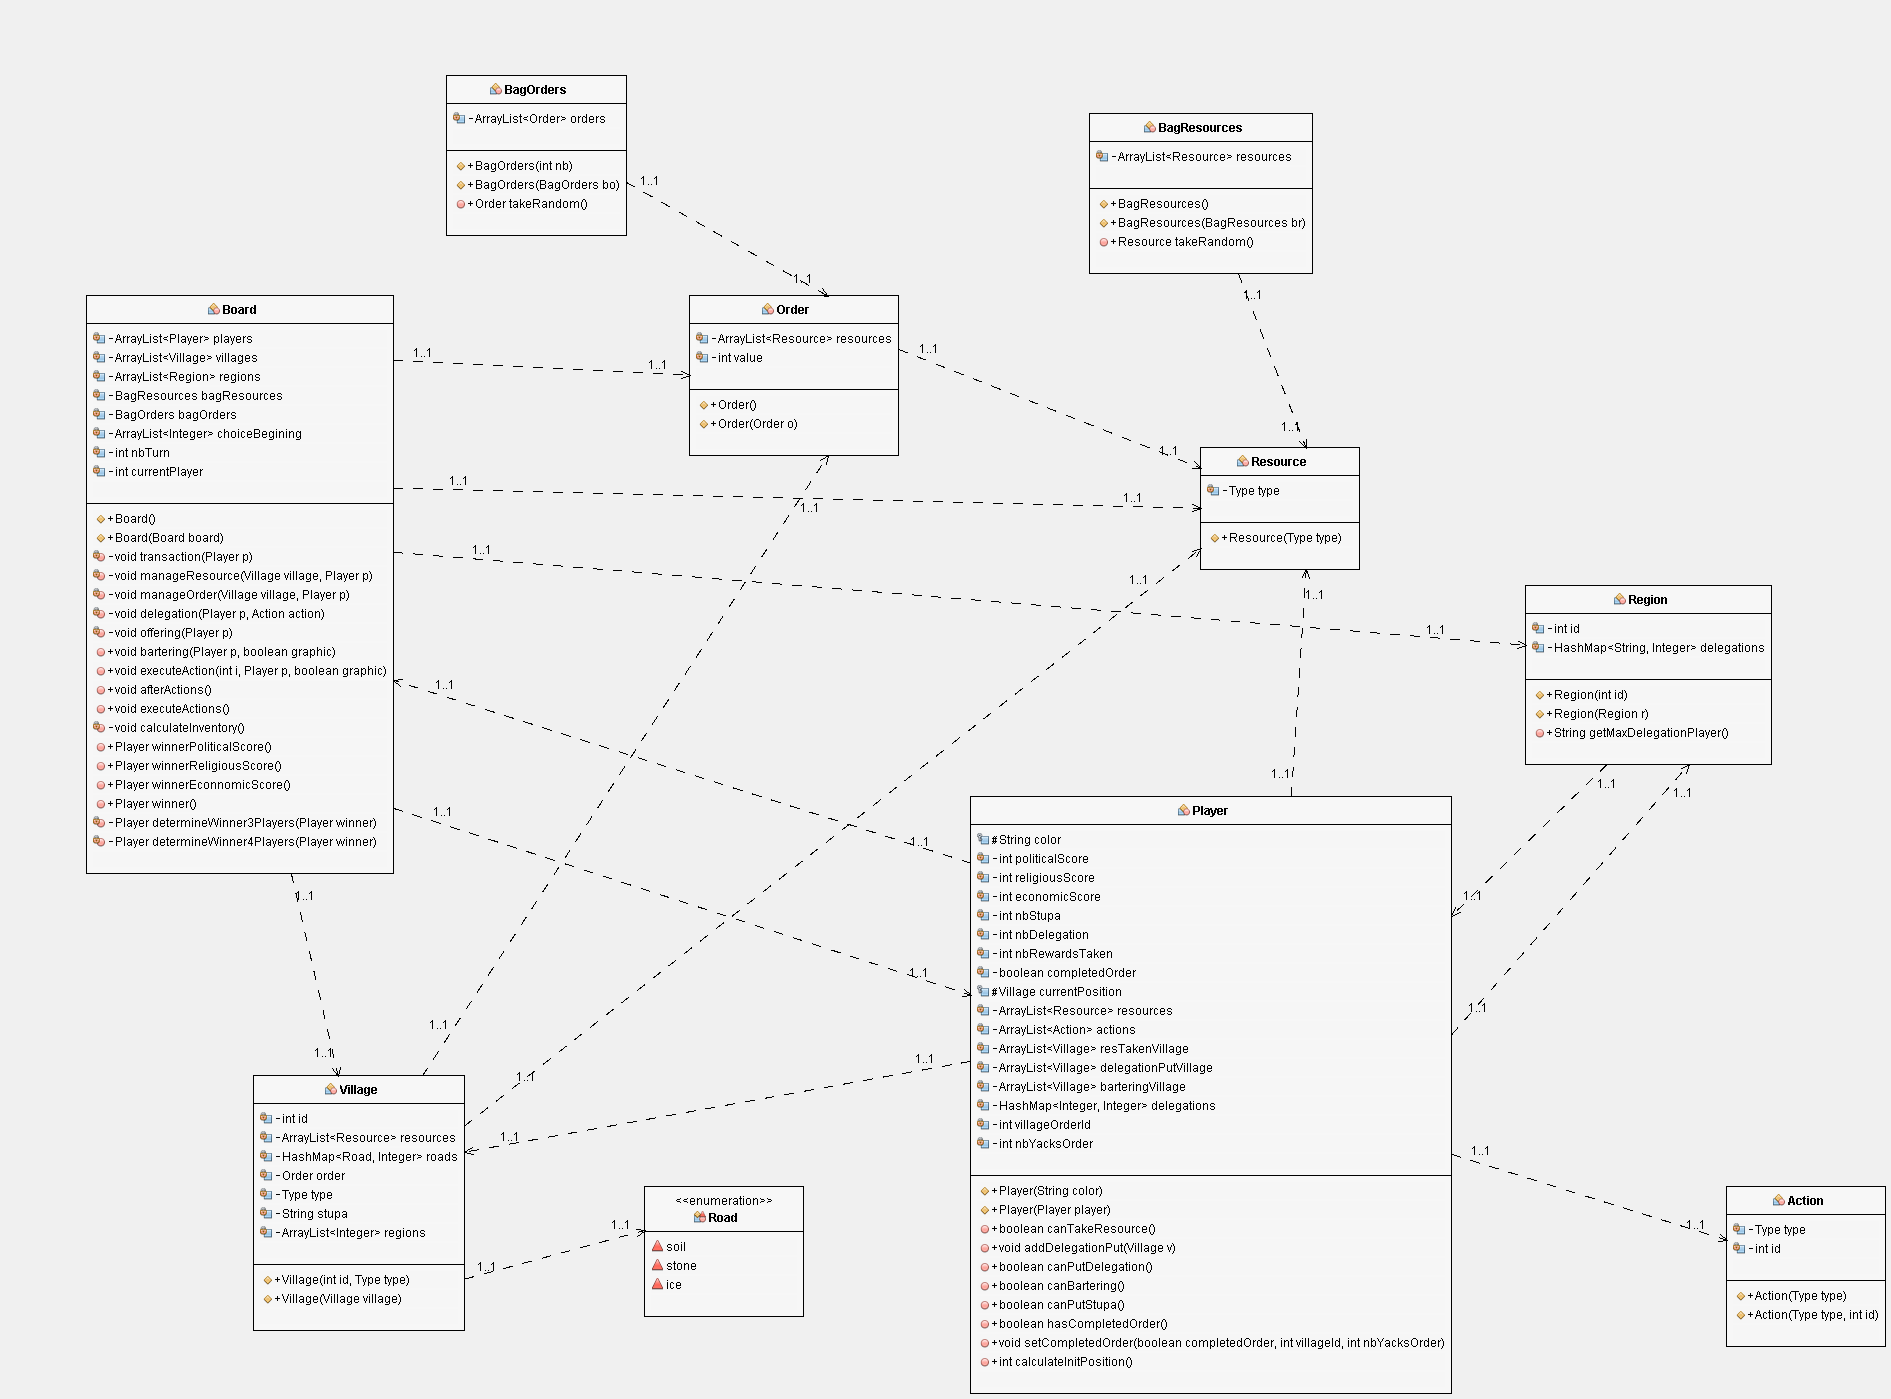
\includegraphics[width=1\linewidth]{images/UML_Himalaya_CORE_3}
	\caption{UML Moteur du jeu version 3.0 après développement}
	\label{fig:UMLCore2}
\end{figure}
\begin{figure}[h]
	\centering
	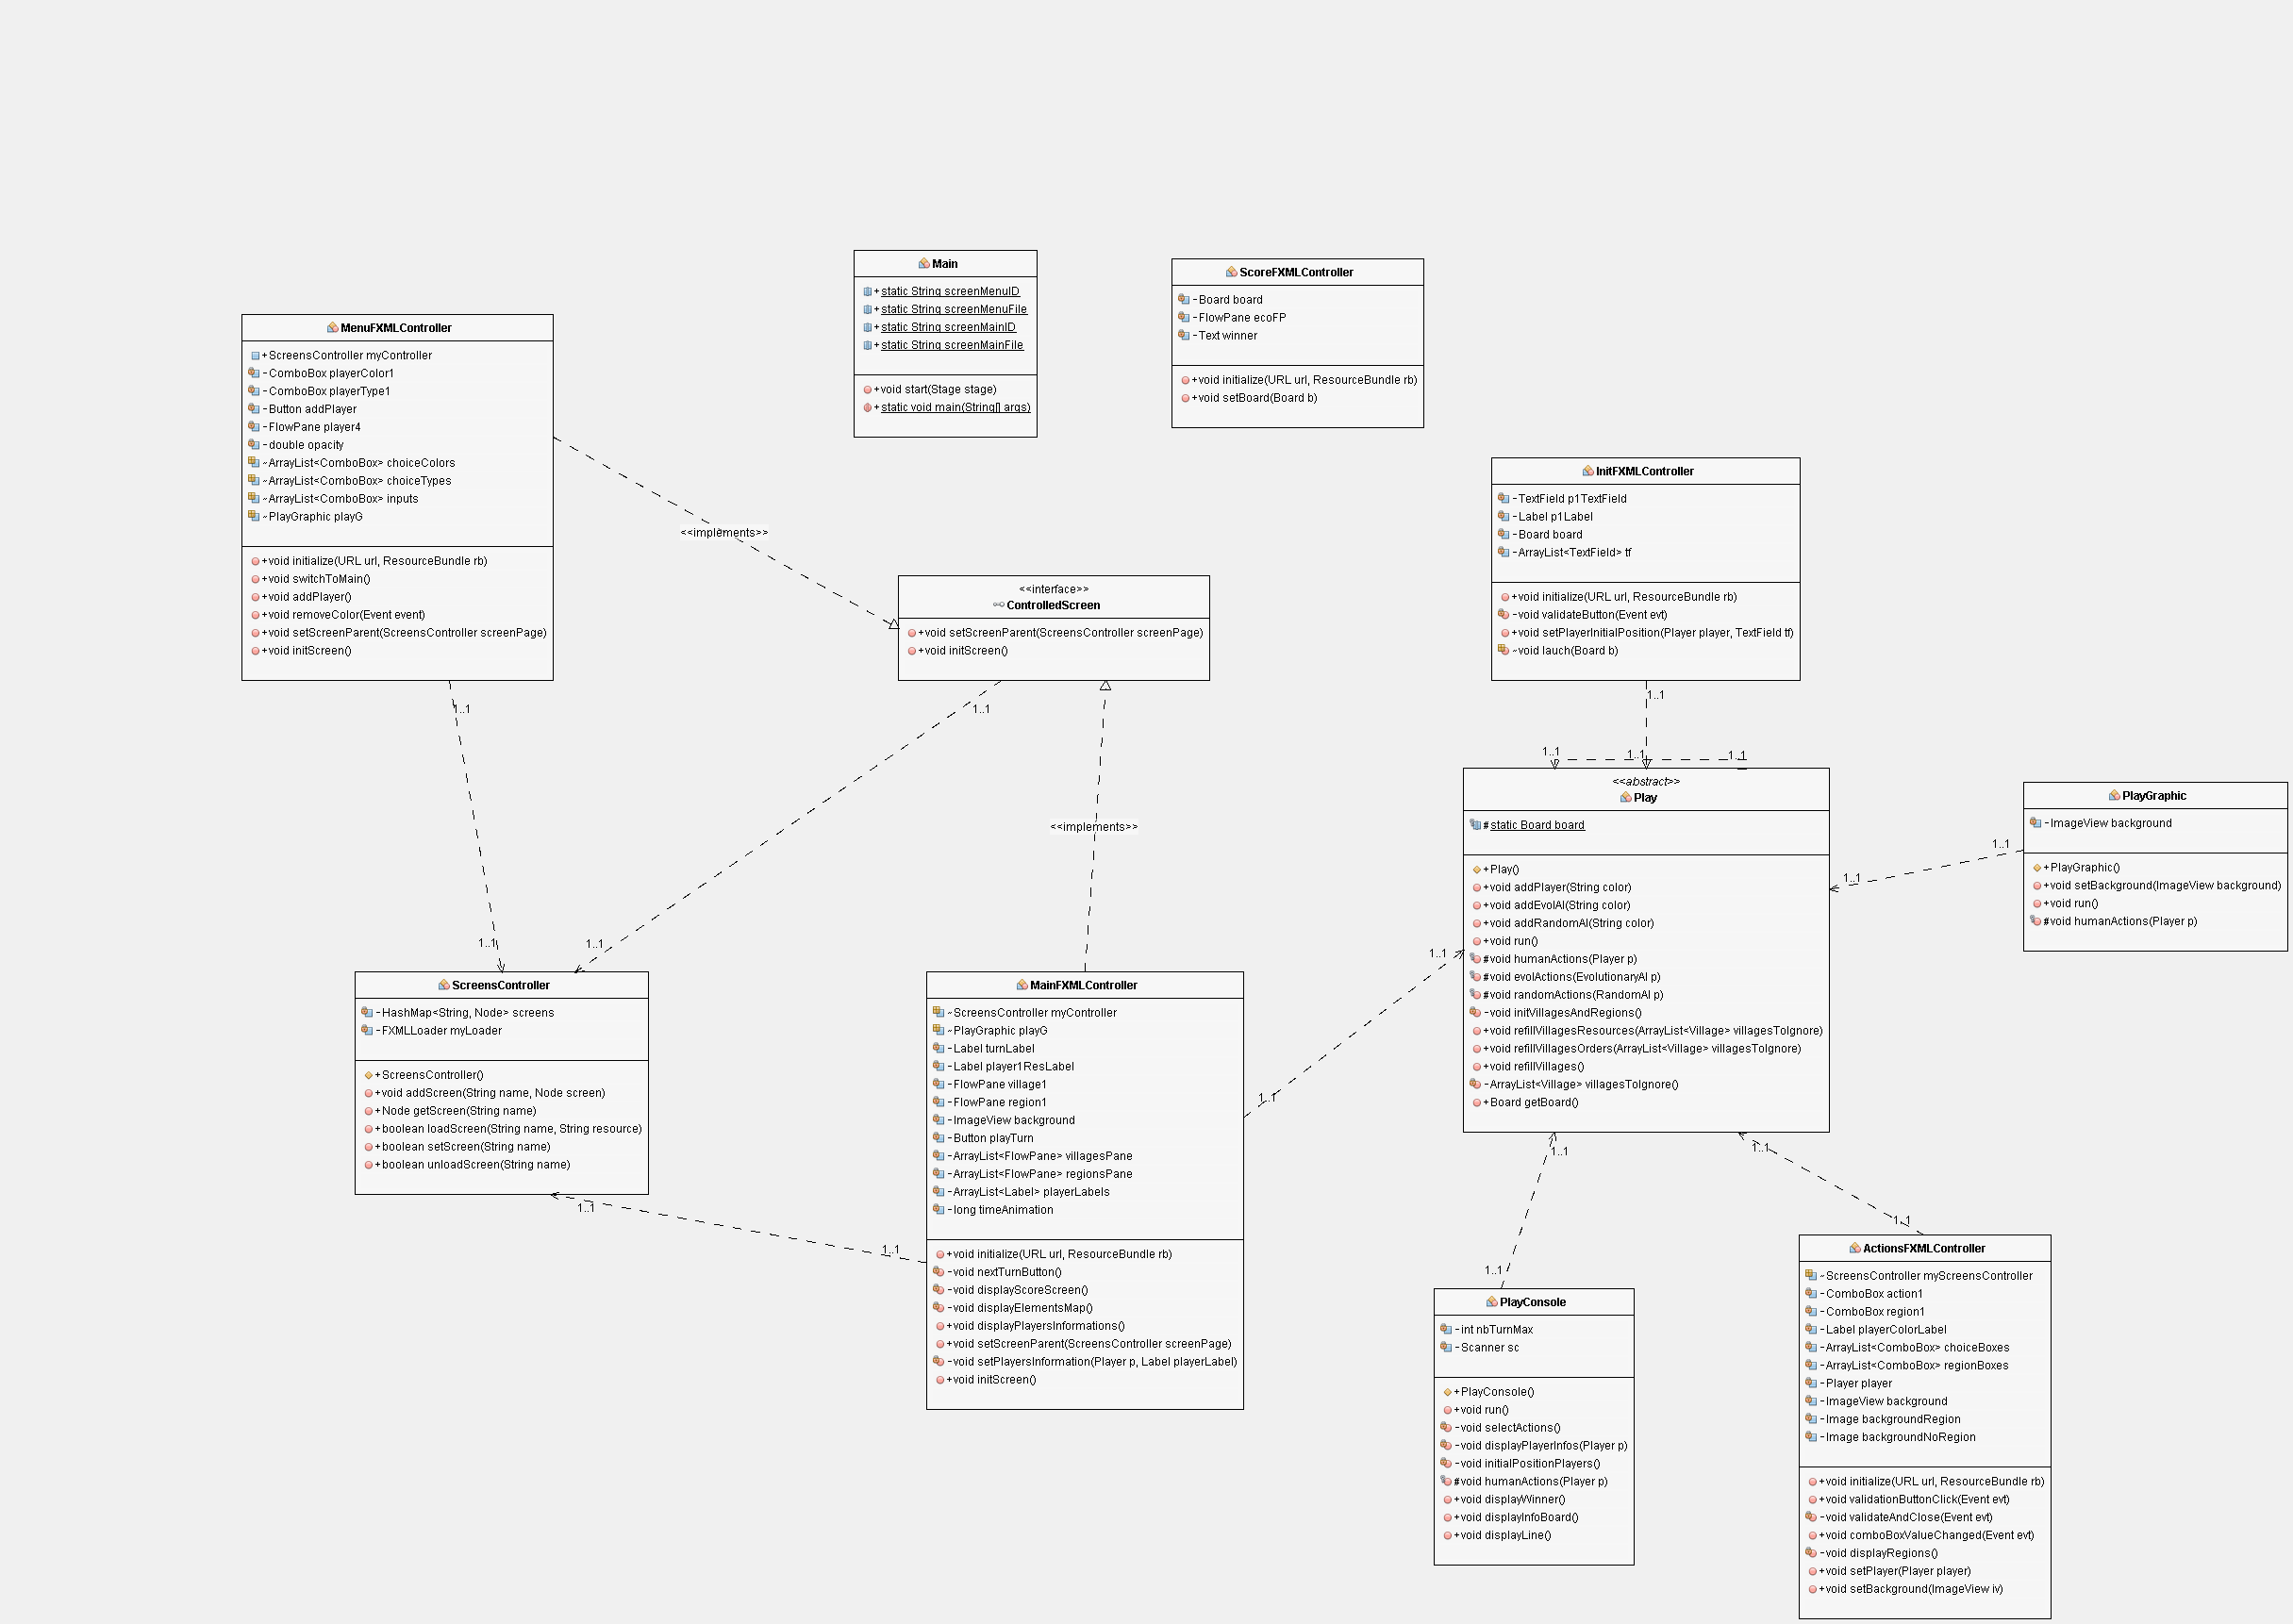
\includegraphics[width=1\linewidth]{images/UML_Himalaya_IHM_1}
	\caption{UML de l'IHM 1.0 après développement}
	\label{fig:UML_IHM}
\end{figure}
\begin{figure}[h]
	\centering
	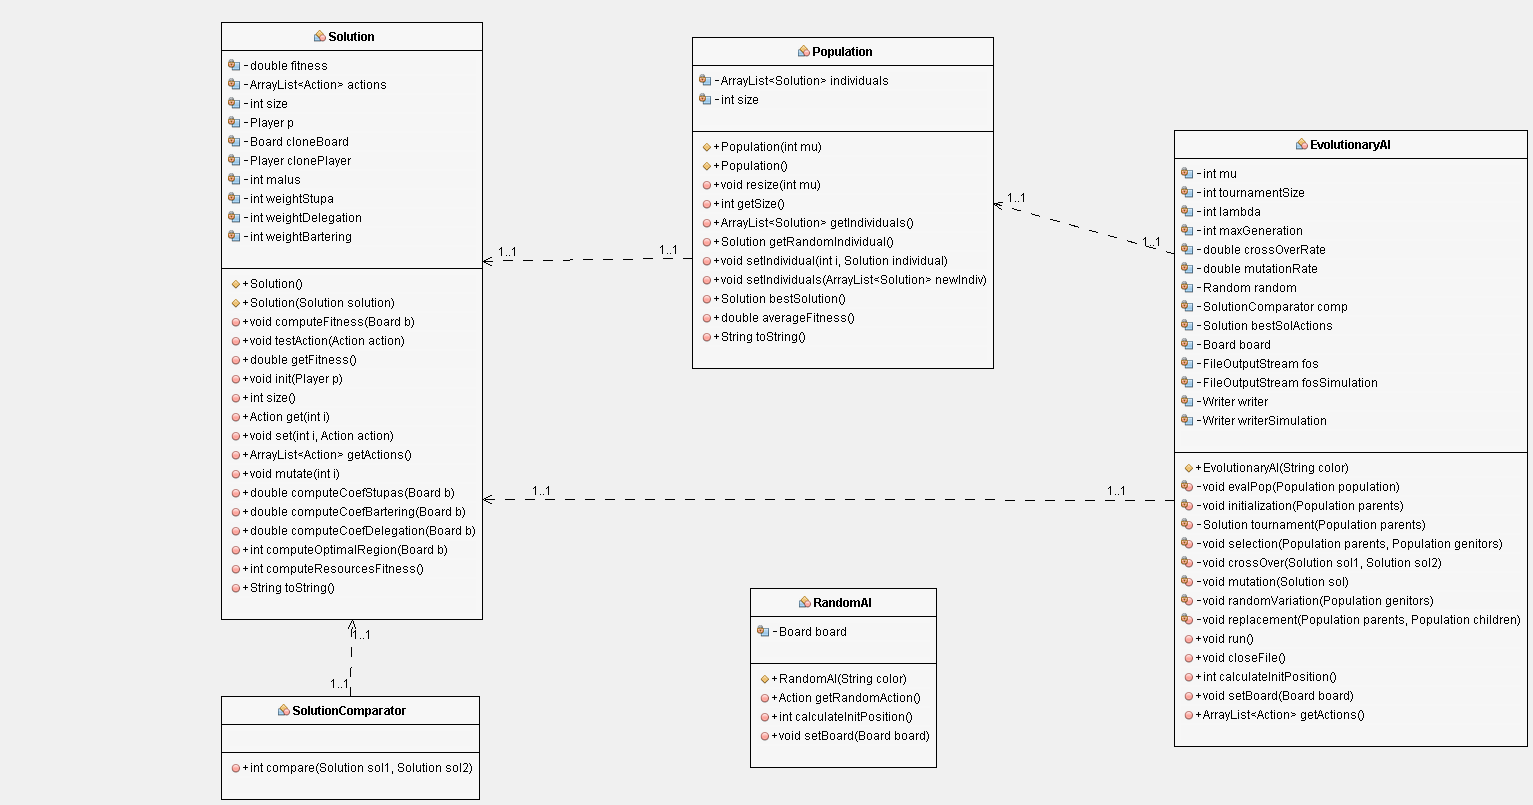
\includegraphics[width=1\linewidth]{images/UML_Himalaya_IA_1}
	\caption{UML de l'IA 1.0 après développement}
	\label{fig:UML_IA}
\end{figure}





\end{document}          
